\documentclass[11pt,a4paper]{article}

% Packages
\usepackage[utf8]{inputenc}
\usepackage[T1]{fontenc}
\usepackage{amsmath,amssymb}
\usepackage{geometry}
\usepackage{graphicx}
\usepackage{xcolor}
\usepackage{listings}
\usepackage{hyperref}
\usepackage{tcolorbox}
\usepackage{enumitem}
\usepackage{tikz}
\usepackage{fancyhdr}
\usepackage{titlesec}

% Page geometry
\geometry{margin=1in}

% Colors
\definecolor{codegreen}{rgb}{0,0.6,0}
\definecolor{codegray}{rgb}{0.5,0.5,0.5}
\definecolor{codepurple}{rgb}{0.58,0,0.82}
\definecolor{backcolour}{rgb}{0.95,0.95,0.92}
\definecolor{keywordblue}{rgb}{0.13,0.13,1}
\definecolor{sectionblue}{RGB}{70,130,180}
\definecolor{highlightgreen}{RGB}{34,139,34}
\definecolor{warningred}{RGB}{220,20,60}
\definecolor{infobox}{RGB}{230,243,255}

% Code listing style
\lstdefinestyle{jsstyle}{
    backgroundcolor=\color{backcolour},
    commentstyle=\color{codegreen},
    keywordstyle=\color{keywordblue}\bfseries,
    numberstyle=\tiny\color{codegray},
    stringstyle=\color{codepurple},
    basicstyle=\ttfamily\footnotesize,
    breakatwhitespace=false,
    breaklines=true,
    captionpos=b,
    keepspaces=true,
    numbers=left,
    numbersep=5pt,
    showspaces=false,
    showstringspaces=false,
    showtabs=false,
    tabsize=2,
    language=Java,
    morekeywords={const,let,async,await,Promise,setTimeout,setInterval,console,log,then,catch,finally,resolve,reject}
}

\lstset{style=jsstyle}

% Box environments
\newtcolorbox{keyconceptbox}[1][]{
    colback=infobox,
    colframe=sectionblue,
    fonttitle=\bfseries,
    title=#1,
    boxrule=1pt,
    arc=3pt
}

\newtcolorbox{warningbox}[1][]{
    colback=red!5,
    colframe=warningred,
    fonttitle=\bfseries,
    title=#1,
    boxrule=1pt,
    arc=3pt
}

\newtcolorbox{definitionbox}[1][]{
    colback=green!5,
    colframe=highlightgreen,
    fonttitle=\bfseries,
    title=#1,
    boxrule=1pt,
    arc=3pt
}

% Header/Footer
\pagestyle{fancy}
\fancyhf{}
\rhead{JavaScript Concurrency Model}
\lhead{Software Engineering - CSEN 303}
\rfoot{Page \thepage}

% Title formatting
\titleformat{\section}
{\color{sectionblue}\normalfont\Large\bfseries}
{\thesection}{1em}{}

\titleformat{\subsection}
{\color{sectionblue}\normalfont\large\bfseries}
{\thesubsection}{1em}{}

% Document
\begin{document}

% Title Page
\begin{titlepage}
    \centering
    \vspace*{2cm}

    {\Huge\bfseries Asynchronous Programming:\\[0.3cm]
    \color{sectionblue}The JavaScript Concurrency Model\par}

    \vspace{1.5cm}

    {\Large Software Engineering - CSEN 303\par}

    \vspace{2cm}

    {\large A Comprehensive Study Guide\par}

    \vspace{3cm}

    \begin{tcolorbox}[colback=gray!10,colframe=gray!50,width=0.8\textwidth]
    \centering
    \textbf{Learning Objectives:}
    \begin{itemize}[leftmargin=*]
        \item Understand JavaScript's single-threaded, non-blocking nature
        \item Differentiate between processes and threads
        \item Master the Event Loop mechanism
        \item Understand the Call Stack, Web APIs, and Callback Queues
        \item Learn execution flow and task prioritization
    \end{itemize}
    \end{tcolorbox}

    \vfill

    {\large Based on lectures by Dr. Iman Awaad\\
    German International University (GIU)\par}

\end{titlepage}

\tableofcontents
\newpage

% =============================================================================
\section{The Nature of JavaScript}
% =============================================================================

JavaScript is fundamentally different from many other programming languages. Understanding its core nature is essential before diving into its concurrency model.

\begin{keyconceptbox}[JavaScript Core Characteristics]
JavaScript is a:
\begin{itemize}
    \item \textbf{High-level} language
    \item \textbf{Asynchronous} language
    \item \textbf{Non-blocking} language
    \item \textbf{Single-threaded} language
    \item \textbf{Interpreted \& JIT compiled} language
    \item \textbf{Concurrent} language
\end{itemize}
\end{keyconceptbox}

\subsection{High-Level Language}

JavaScript provides significant abstraction from underlying computer hardware:

\begin{center}
\begin{tabular}{|l|l|}
\hline
\textbf{Level} & \textbf{Description} \\
\hline
Machine Language & No abstraction: \texttt{01010101000111} \\
\hline
Low-level Language & One level of abstraction: Assembly code \\
\hline
High-level Language & C, Java, JS, Python, LISP, etc. \\
\hline
\end{tabular}
\end{center}

\subsection{Why Single-Threaded Yet Non-Blocking?}

This seems contradictory! How can JavaScript:
\begin{itemize}
    \item Execute only \textbf{one piece of code at a time}
    \item Yet \textbf{not freeze} when waiting for long operations?
\end{itemize}

\begin{warningbox}[The Problem]
If JavaScript were synchronous and blocking, operations like:
\begin{itemize}
    \item Fetching data from an API
    \item Database operations
    \item File I/O
    \item User interactions
\end{itemize}
Would \textbf{freeze the entire application} until they complete!
\end{warningbox}

\begin{definitionbox}[The Solution: Asynchronous, Event-Driven Model]
JavaScript achieves concurrency through an \textbf{asynchronous, event-driven model} rather than true parallelism. This provides the \textit{illusion of simultaneous execution} while maintaining a single thread of execution.
\end{definitionbox}

\subsection{Synchronous vs Asynchronous Execution}

\textbf{Synchronous execution:}
\begin{lstlisting}
// Each operation must complete before the next begins
console.log("log1");
console.log("log2");
console.log("log3");
// Output: log1, log2, log3 (in order)
\end{lstlisting}

\textbf{Asynchronous execution:}
\begin{lstlisting}
console.log("log1");
setTimeout(() => {
    console.log("log2");
}, 1000);
console.log("log3");
// Output: log1, log3, log2 (log2 appears after 1 second)
\end{lstlisting}

\begin{keyconceptbox}[Key Insight]
In asynchronous execution:
\begin{enumerate}
    \item Operations are \textbf{started} quickly
    \item \textbf{Responses} arrive later, in any order
    \item The main thread continues executing other code
\end{enumerate}
\end{keyconceptbox}

\newpage
% =============================================================================
\section{The Architecture: Processes vs Threads}
% =============================================================================

Understanding the difference between processes and threads explains why JavaScript is considered "lightweight" but why blocking the main thread is dangerous.

\subsection{Process}

\begin{definitionbox}[Process]
An \textbf{executing program loaded into memory}.
\end{definitionbox}

\textbf{Characteristics:}
\begin{itemize}
    \item Has its own \textbf{distinct memory space} and resources
    \item Operates in \textbf{isolation} from other processes
    \item Considered \textbf{"heavyweight"} operations
    \item Requires more time and resources to create/terminate
    \item \textbf{Fault tolerant}: failure in one process unlikely to affect others
\end{itemize}

\subsection{Thread}

\begin{definitionbox}[Thread]
The \textbf{basic unit of execution within a process} (also called "lightweight process").
\end{definitionbox}

\textbf{Characteristics:}
\begin{itemize}
    \item Threads in the same process \textbf{share memory} and resources
    \item Allows for \textbf{faster, more efficient communication}
    \item \textbf{Risk}: An error in one thread can crash the entire parent process
\end{itemize}

\subsection{Visual Comparison}

\begin{center}
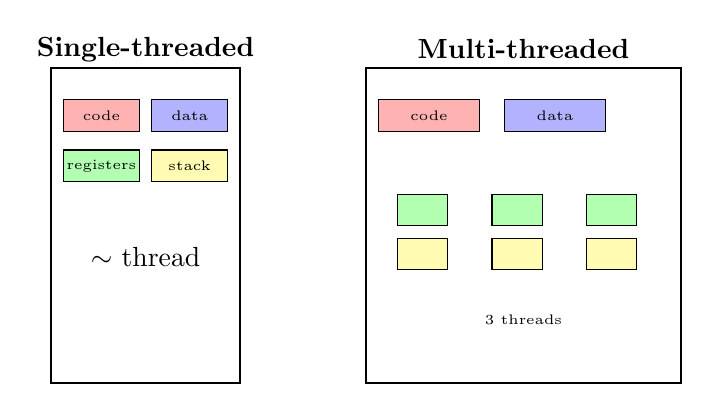
\begin{tikzpicture}[scale=0.8]
    % Single-threaded process
    \draw[thick] (0,0) rectangle (3,5);
    \node at (1.5,5.3) {\textbf{Single-threaded}};

    % Components
    \draw[fill=red!30] (0.2,4) rectangle (1.4,4.5);
    \node[font=\tiny] at (0.8,4.25) {code};

    \draw[fill=blue!30] (1.6,4) rectangle (2.8,4.5);
    \node[font=\tiny] at (2.2,4.25) {data};

    \draw[fill=green!30] (0.2,3.2) rectangle (1.4,3.7);
    \node[font=\tiny] at (0.8,3.45) {registers};

    \draw[fill=yellow!30] (1.6,3.2) rectangle (2.8,3.7);
    \node[font=\tiny] at (2.2,3.45) {stack};

    \node at (1.5,2) {$\sim$ thread};

    % Multi-threaded process
    \draw[thick] (5,0) rectangle (10,5);
    \node at (7.5,5.3) {\textbf{Multi-threaded}};

    % Shared components
    \draw[fill=red!30] (5.2,4) rectangle (6.8,4.5);
    \node[font=\tiny] at (6,4.25) {code};

    \draw[fill=blue!30] (7.2,4) rectangle (8.8,4.5);
    \node[font=\tiny] at (8,4.25) {data};

    % Multiple threads
    \foreach \x in {5.5,7,8.5} {
        \draw[fill=green!30] (\x,2.5) rectangle (\x+0.8,3);
        \draw[fill=yellow!30] (\x,1.8) rectangle (\x+0.8,2.3);
    }
    \node[font=\tiny] at (7.5,1) {3 threads};
\end{tikzpicture}
\end{center}

\begin{keyconceptbox}[JavaScript's Approach]
JavaScript executes \textbf{one piece of code at a time on a single call stack}. It does everything within a \textbf{single process}!

This means:
\begin{itemize}
    \item Lightweight and efficient
    \item But blocking the main thread freezes everything
    \item Solution: The Event Loop mechanism
\end{itemize}
\end{keyconceptbox}

\newpage
% =============================================================================
\section{The Mechanism: The Event Loop}
% =============================================================================

The Event Loop is JavaScript's mechanism for handling multiple tasks concurrently despite being single-threaded.

\subsection{The Call Stack}

\begin{definitionbox}[Call Stack]
A \textbf{LIFO (Last-In-First-Out)} data structure that tracks function execution.
\end{definitionbox}

\subsubsection{Stack Operations}

\begin{center}
\begin{tabular}{|l|l|}
\hline
\textbf{Operation} & \textbf{Description} \\
\hline
\texttt{push} & Add a new piece of data to the top \\
\hline
\texttt{pop} & Remove data from the top \\
\hline
\texttt{top/peek} & Look at top data without removing \\
\hline
\texttt{isEmpty} & Check if stack is empty \\
\hline
\end{tabular}
\end{center}

\textbf{Example:}
\begin{lstlisting}
function multiply(a, b) {
    return a * b;
}

function square(n) {
    return multiply(n, n);
}

function printSquare(n) {
    let result = square(n);
    console.log(result);
}

printSquare(4);
\end{lstlisting}

\textbf{Call Stack progression:}
\begin{enumerate}
    \item \texttt{printSquare(4)} pushed
    \item \texttt{square(4)} pushed
    \item \texttt{multiply(4, 4)} pushed
    \item \texttt{multiply} returns 16, popped
    \item \texttt{square} returns 16, popped
    \item \texttt{console.log(16)} pushed, executed, popped
    \item \texttt{printSquare} completes, popped
\end{enumerate}

\subsection{Web APIs}

\begin{definitionbox}[Web APIs]
Interfaces exposed by web browsers that allow JavaScript code to interact with various browser functionalities and system resources. They are \textbf{NOT part of the core JavaScript language} but are provided by the browser environment.
\end{definitionbox}

Web APIs:
\begin{itemize}
    \item Guarantee \textbf{availability} of operations
    \item Guarantee \textbf{input and output types}
\end{itemize}

\subsubsection{Examples of Web APIs}

\begin{center}
\begin{tabular}{|p{4cm}|p{8cm}|}
\hline
\textbf{API} & \textbf{Description} \\
\hline
DOM API & Interact with page structure, style, content \\
& e.g., \texttt{document.getElementById()}, \texttt{addEventListener()} \\
\hline
Fetch API & Make network requests (e.g., fetching data from server) \\
\hline
Web Storage APIs & Store data locally (LocalStorage, SessionStorage) \\
\hline
Multimedia APIs & Work with audio, video, media elements \\
\hline
Geolocation API & Request user's geographical location \\
\hline
Notification API & Display system notifications \\
\hline
Clipboard API & Access system clipboard \\
\hline
\end{tabular}
\end{center}

\begin{keyconceptbox}[How Web APIs Enable Async]
When a long-running operation (like \texttt{setTimeout} or \texttt{fetch}) is encountered:
\begin{enumerate}
    \item It's handed off to the browser's Web APIs
    \item JavaScript continues executing other code
    \item When the operation completes, its callback goes to a queue
\end{enumerate}
\end{keyconceptbox}

\subsection{The Queues}

JavaScript has two types of queues for handling asynchronous callbacks:

\subsubsection{Callback Queue (Macrotask Queue / Task Queue)}

\begin{definitionbox}[Callback Queue]
Holds callbacks from \textbf{standard asynchronous operations}.
\end{definitionbox}

\textbf{Sources:}
\begin{itemize}
    \item \texttt{setTimeout()}, \texttt{setInterval()}
    \item \texttt{setImmediate()} (Node.js)
    \item I/O operations (network requests, file system)
    \item User events (mouse clicks, keyboard input)
\end{itemize}

\subsubsection{Microtask Queue}

\begin{definitionbox}[Microtask Queue]
Holds callbacks from \textbf{higher-priority asynchronous operations}.
\end{definitionbox}

\textbf{Sources:}
\begin{itemize}
    \item Promise callbacks: \texttt{.then()}, \texttt{.catch()}, \texttt{.finally()}
    \item \texttt{MutationObserver} callbacks
    \item \texttt{process.nextTick()} (Node.js)
\end{itemize}

\subsubsection{Key Differences}

\begin{center}
\begin{tabular}{|p{3cm}|p{5cm}|p{5cm}|}
\hline
\textbf{Aspect} & \textbf{Callback Queue} & \textbf{Microtask Queue} \\
\hline
Priority & Lower & \textbf{Higher} \\
\hline
Contents & General async operations & Promise-related operations \\
\hline
Processing & One task per loop iteration & \textbf{All tasks} before next macrotask \\
\hline
\end{tabular}
\end{center}

\newpage
% =============================================================================
\section{Execution Flow: The Event Loop Algorithm}
% =============================================================================

\begin{keyconceptbox}[Event Loop Algorithm]
The Event Loop follows this cycle:
\begin{enumerate}
    \item Execute all synchronous code (until Call Stack is empty)
    \item Check the \textbf{Microtask Queue}
    \begin{itemize}
        \item Execute \textbf{ALL} microtasks until queue is empty
    \end{itemize}
    \item Check the \textbf{Callback Queue (Macrotask Queue)}
    \begin{itemize}
        \item Execute \textbf{ONE} macrotask
    \end{itemize}
    \item Repeat from step 2
\end{enumerate}
\end{keyconceptbox}

\subsection{Priority in Action}

\begin{lstlisting}
console.log("Start");

setTimeout(() => {
    console.log("Timeout callback (Macrotask)");
}, 0);

Promise.resolve().then(() => {
    console.log("Promise callback (Microtask)");
});

console.log("End");
\end{lstlisting}

\textbf{Output:}
\begin{lstlisting}[numbers=none]
Start
End
Promise callback (Microtask)
Timeout callback (Macrotask)
\end{lstlisting}

\textbf{Explanation:}
\begin{enumerate}
    \item \texttt{console.log("Start")} - synchronous, executes immediately
    \item \texttt{setTimeout} - callback sent to Web APIs, then to Callback Queue
    \item \texttt{Promise.resolve().then()} - callback goes to Microtask Queue
    \item \texttt{console.log("End")} - synchronous, executes immediately
    \item Call Stack empty $\rightarrow$ process Microtask Queue first
    \item Promise callback executes
    \item Microtask Queue empty $\rightarrow$ process one from Callback Queue
    \item setTimeout callback executes
\end{enumerate}

\begin{warningbox}[Important]
Even with \texttt{setTimeout(..., 0)}, the callback goes through the Callback Queue and must wait for:
\begin{itemize}
    \item All synchronous code to complete
    \item All microtasks to be processed
\end{itemize}
\end{warningbox}

\subsection{Callbacks: The Foundation}

\begin{definitionbox}[Callback]
A function passed as an argument to another function, to be executed later when an asynchronous operation completes.
\end{definitionbox}

\begin{lstlisting}
function fetchData(callback) {
    // Simulate async operation
    setTimeout(() => {
        const data = "Some fetched data";
        callback(data); // Execute callback with data
    }, 2000);
}

function processData(data) {
    console.log("Processing:", data);
}

fetchData(processData);
console.log("Data fetching initiated...");

// Output:
// Data fetching initiated...
// (2 seconds later)
// Processing: Some fetched data
\end{lstlisting}

\subsection{Promises: Better Async Handling}

\begin{definitionbox}[Promise]
An object representing the eventual completion (or failure) of an asynchronous operation and its resulting value.
\end{definitionbox}

Promises provide a more structured way to handle async code compared to nested callbacks (avoiding "callback hell").

\begin{lstlisting}
const myPromise = new Promise((resolve, reject) => {
    // Async operation
    setTimeout(() => {
        const success = true;
        if (success) {
            resolve("Operation successful!");
        } else {
            reject("Operation failed!");
        }
    }, 1000);
});

myPromise
    .then(result => console.log(result))
    .catch(error => console.error(error))
    .finally(() => console.log("Cleanup"));
\end{lstlisting}

\subsection{Async/Await: Syntactic Sugar}

\begin{definitionbox}[async/await]
Syntactic sugar built on top of Promises that makes asynchronous code look and behave more like synchronous code.
\end{definitionbox}

\begin{lstlisting}
async function fetchUserData() {
    try {
        const response = await fetch('/api/user');
        const data = await response.json();
        console.log(data);
    } catch (error) {
        console.error("Error:", error);
    }
}

// async functions always return a Promise
// await pauses execution until the Promise settles
\end{lstlisting}

\newpage
% =============================================================================
\section{JavaScript Runtime Environment}
% =============================================================================

\begin{center}
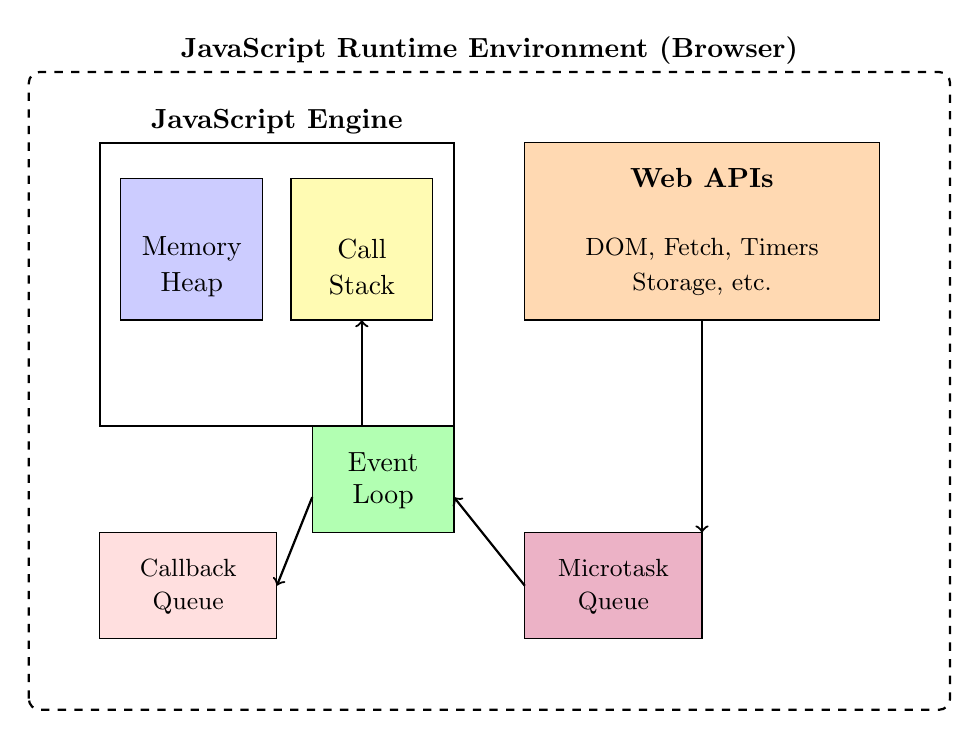
\begin{tikzpicture}[scale=0.9]
    % Main container
    \draw[thick, dashed, rounded corners] (-1,-1) rectangle (12,8);
    \node at (5.5,8.3) {\textbf{JavaScript Runtime Environment (Browser)}};

    % JavaScript Engine
    \draw[thick] (0,3) rectangle (5,7);
    \node at (2.5,7.3) {\textbf{JavaScript Engine}};

    % Memory Heap
    \draw[fill=blue!20] (0.3,4.5) rectangle (2.3,6.5);
    \node at (1.3,5.5) {Memory};
    \node at (1.3,5) {Heap};

    % Call Stack
    \draw[fill=yellow!30] (2.7,4.5) rectangle (4.7,6.5);
    \node at (3.7,5.5) {Call};
    \node at (3.7,5) {Stack};

    % Web API
    \draw[fill=orange!30] (6,4.5) rectangle (11,7);
    \node at (8.5,6.5) {\textbf{Web APIs}};
    \node[font=\small] at (8.5,5.5) {DOM, Fetch, Timers};
    \node[font=\small] at (8.5,5) {Storage, etc.};

    % Event Loop
    \draw[fill=green!30] (3,1.5) rectangle (5,3);
    \node at (4,2.5) {Event};
    \node at (4,2) {Loop};

    % Callback Queue
    \draw[fill=pink!50] (0,0) rectangle (2.5,1.5);
    \node[font=\small] at (1.25,1) {Callback};
    \node[font=\small] at (1.25,0.5) {Queue};

    % Microtask Queue
    \draw[fill=purple!30] (6,0) rectangle (8.5,1.5);
    \node[font=\small] at (7.25,1) {Microtask};
    \node[font=\small] at (7.25,0.5) {Queue};

    % Arrows
    \draw[->, thick] (8.5,4.5) -- (8.5,1.5);
    \draw[->, thick] (6,0.75) -- (5,2);
    \draw[->, thick] (3,2) -- (2.5,0.75);
    \draw[->, thick] (3.7,3) -- (3.7,4.5);

\end{tikzpicture}
\end{center}

\subsection{Flow Summary}

\begin{enumerate}
    \item Code enters the \textbf{Call Stack} for execution
    \item When async operations are encountered, they're sent to \textbf{Web APIs}
    \item Web APIs handle the operations (timers, network requests, etc.)
    \item Once complete, callbacks go to appropriate queue:
    \begin{itemize}
        \item Promises $\rightarrow$ Microtask Queue
        \item Timers, I/O $\rightarrow$ Callback Queue
    \end{itemize}
    \item \textbf{Event Loop} checks if Call Stack is empty
    \item If empty: drain Microtask Queue, then one from Callback Queue
    \item Repeat
\end{enumerate}

\newpage
% =============================================================================
\section{Web Workers: True Parallelism}
% =============================================================================

\begin{definitionbox}[Web Workers]
Provide a form of \textbf{multi-threading in the browser} by allowing scripts to run in the background in separate threads.
\end{definitionbox}

\textbf{Key Points:}
\begin{itemize}
    \item Run in separate threads (true parallelism)
    \item Prevent blocking the main UI thread
    \item Communicate with main thread via message passing
    \item Cannot directly access the DOM
\end{itemize}

\begin{warningbox}[Concurrency vs Parallelism]
\begin{itemize}
    \item \textbf{Concurrency} (async/await/event loops): Managing multiple tasks that can make progress without running simultaneously
    \item \textbf{Parallelism} (threads/CPU cores): Actually running multiple tasks at the same time
\end{itemize}

JavaScript's Event Loop provides \textbf{concurrency}, while Web Workers provide \textbf{parallelism}.
\end{warningbox}

\newpage
% =============================================================================
\section{Additional Implementation Details}
% =============================================================================

\subsection{DOM: Document Object Model}

The DOM represents HTML/XML in a tree structure that JavaScript can manipulate:
\begin{itemize}
    \item Methods for selecting HTML elements
    \item Objects with methods and properties
    \item Changes to DOM automatically update HTML
\end{itemize}

\textbf{Key mechanisms:}
\begin{itemize}
    \item Query selectors
    \item Event listeners
    \item Style properties
\end{itemize}

\subsection{jQuery}

A JavaScript library that simplifies:
\begin{itemize}
    \item DOM manipulation across browsers
    \item AJAX requests
    \item UI enhancements (date pickers, sliders, etc.)
    \item Dynamic CSS modification
\end{itemize}

jQuery code starts with \texttt{\$}:
\begin{lstlisting}
$('#myElement').click(function() {
    $(this).hide();
});
\end{lstlisting}

\subsection{AJAX}

\textbf{Asynchronous JavaScript and XML} - technique for exchanging data with a server without reloading the page.

\begin{itemize}
    \item Uses XMLHttpRequest object
    \item Can request text, JSON, HTML, etc.
    \item jQuery simplifies AJAX requests
\end{itemize}

\subsection{Node.js}

JavaScript runtime environment for the server side:
\begin{itemize}
    \item Node.js + HTTP = Express framework
    \item NPM (Node Package Manager) for package management
    \item Same Event Loop model as browser JavaScript
\end{itemize}

\newpage
% =============================================================================
\section{Summary}
% =============================================================================

\begin{keyconceptbox}[Key Takeaways]
\begin{enumerate}
    \item \textbf{JavaScript is single-threaded but non-blocking} through its asynchronous, event-driven model

    \item \textbf{The Event Loop} is the core mechanism enabling concurrency:
    \begin{itemize}
        \item Monitors Call Stack and Queues
        \item Prioritizes Microtasks over Macrotasks
    \end{itemize}

    \item \textbf{Call Stack} executes synchronous code (LIFO)

    \item \textbf{Web APIs} handle long-running operations off the main thread

    \item \textbf{Two Queues}:
    \begin{itemize}
        \item Microtask Queue (Promises) - higher priority
        \item Callback Queue (setTimeout, I/O) - lower priority
    \end{itemize}

    \item \textbf{Execution order}: Sync $\rightarrow$ All Microtasks $\rightarrow$ One Macrotask $\rightarrow$ Repeat

    \item \textbf{Callbacks $\rightarrow$ Promises $\rightarrow$ async/await}: Evolution of async patterns

    \item \textbf{Web Workers} provide true parallelism when needed
\end{enumerate}
\end{keyconceptbox}

\subsection{Useful Tools}

\begin{itemize}
    \item \textbf{Loupe}: \url{https://github.com/latentflip/loupe}
    \begin{itemize}
        \item Visualizes Call Stack, Event Loop, Callback Queue interactions
    \end{itemize}

    \item \textbf{JS Visualizer 9000}: \url{https://www.jsv9000.app/}
    \begin{itemize}
        \item Interactive Event Loop visualization
    \end{itemize}
\end{itemize}

\vfill

\begin{center}
\textit{"I mark the hours everyone\\
Nor have I yet outrun the sun\\
My use and value unto you\\
Are gauged by what you have to do."}\\[0.5em]
- Inscription on Time Turner
\end{center}

\end{document}
